\subsection*{Hypothesis 5}

Hypothesis 5 examines the influence of book categories on review scores.
To test this hypothesis,we considered the rating score as the metric and removed missing values.
two competing hypotheses were established:\\
\textbf{H0 (Null Hypothesis):} Rating scores are not related to the book categories,
as all rating scores are drawn from the same distribution.\\
\textbf{H1 (Alternative Hypothesis):} Rating scores are affected by the book category,
indicating that the rating scores of each category follow different distributions.\\
As in the previous hypothesis, categories with fewer than 20 reviews were omitted for consistency.
An ANOVA (Analysis of Variance) test was conducted to assess the validity of these hypotheses.
The results of the test revealed an F-statistic of 0.177 and a P-value of 0.999.
A low F-statistic value and a P-value close to 1 suggest that there is not much variation
between the means of different categories.
Therefore, we could not reject the null hypothesis (H0) and concluded that book categories
do not significantly impact rating scores.
This result was further supported by the accompanying boxplot (Figure \ref{fig:h5}),
which showed that the distribution of rating scores was similar across categories.
\begin{figure}[H]
    \centering
    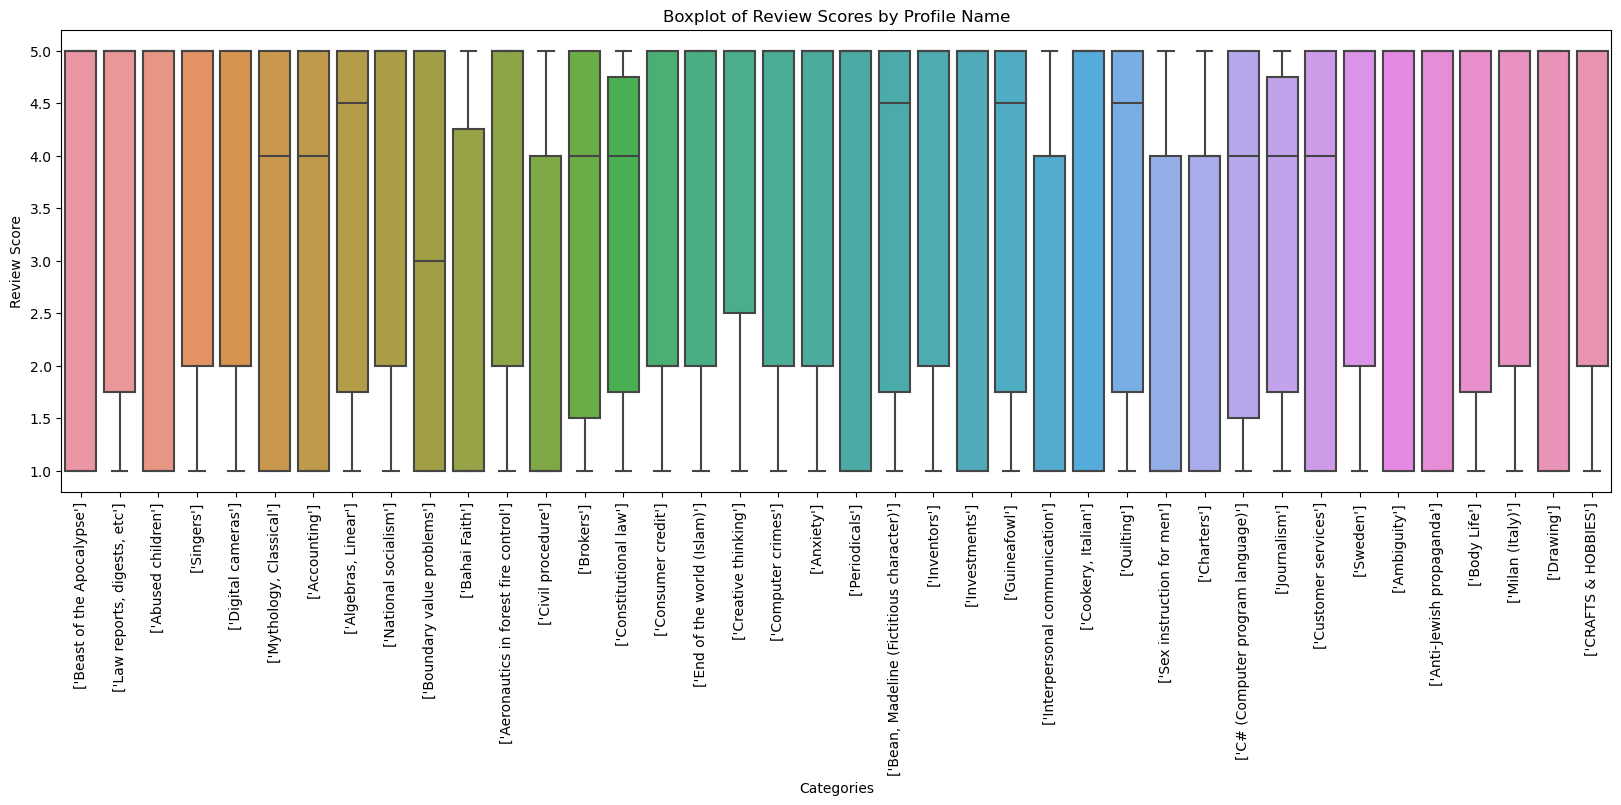
\includegraphics[width=0.5\textwidth]{./figures/h5.png}
    \caption{Distribution of rating scores across categories}
    \label{fig:h5}
\end{figure}
